\chapter{Peliteoria}

Peliteoria etsii tapoja pelata pelejä voitokkaasti.
Tässä luvussa keskitymme kahden pelaajan peleihin,
joissa pelaajat tekevät siirtoja vuorotellen.
Osoittautuu, että monia tällaisia pelejä voi mallintaa
nim-pelin avulla, johon on olemassa yksinkertainen
voittostrategia.

\section{Pelin tila}

Pelin tila kertoo, missä vaiheessa peli on
sillä hetkellä. Jokaiseen tilaan liittyy
mahdollisia siirtoja, jotka johtavat toisiin tiloihin.
Tavoitteena on usein laskea pelin tilasta,
kumpi pelaaja voittaa, jos molemmat pelaavat
optimaalisesti.
Tutustumme seuraavaksi kahteen usein esiintyvään pelityyppiin.


\subsection{Voitto ja häviö}

Monissa peleissä pelaajat tekevät siirtoja
vuorotellen, kunnes siirtoa ei pysty enää tekemään.
Pelistä riippuen viimeisen siirron tekijä
voittaa tai häviää pelin.
Näin on esimerkiksi seuraavassa pelissä:

\textit{Tikkupeli:} Pöydällä on $n$ tikkua kasassa,
ja pelaajat poistavat vuorotellen kasasta tikkuja.
Pelaaja saa poistaa kerrallaan 1, 2 tai 3 tikkua.
Pelin voittaa se, joka poistaa viimeisen tikun.

Tällaisessa pelissä jokainen pelin tila on joko
voittotila tai häviötila.
Voittotilassa oleva pelaaja pystyy
voittamaan pelin,
ja häviötilassa oleva pelaaja häviää pelin,
jos vastustaja toimii optimaalisesti.

Tikkupelissä pelin tila on tikkujen määrä pöydällä.
Tila 0 on häviötila, koska tikkuja ei voi poistaa.
Tilat 1, 2 ja 3 ovat voittotiloja,
koska niissä voi poistaa 1, 2 tai 3 tikkua,
jolloin vastustaja häviää pelin.
Tila 4 on taas häviötila, koska 1, 2 tai 3 tikun
poistaminen johtaa tilaan,
joka on vastustajalle voittotila.

Seuraava taulukko näyttää tikkupelin tilojen luokittelun,
kun tikkuja on $0,1,\ldots,15$.
Merkki V tarkoittaa voittotilaa ja merkki H tarkoittaa häviötilaa.

\begin{center}
\begin{tabular}{rrrrrrrrrrrrrrrr}
0 & 1 & 2 & 3 & 4 & 5 & 6 & 7 & 8 & 9 & 10 & 11 & 12 & 13 & 14 & 15\\
\hline
H & V & V & V & H & V & V & V & H & V & V & V & H & V & V & V \\
\end{tabular}
\end{center}

Kuten taulukosta voi huomata,
tikkupelissä on helppoa päätellä,
onko tila voittotila vai häviötila.
Jos kasassa on 4:llä jaollinen määrä tikkuja,
tila on häviötila,
ja muuten tila on voittotila.

Yleisessä tapauksessa pätee, että tila on
voittotila, jos siitä pääsee jollakin siirrolla häviötilaan,
ja tila on häviötila,
jos kaikki mahdolliset siirrot vievät voittotiloihin.
Tällä päättelyllä pystyy luokittelemaan minkä tahansa vastaavan
pelin tilat voitto- ja häviötiloihin.

\subsection{Pisteiden keräys}

Joissakin peleissä pelaajat keräävät pisteitä
pelin aikana ja tavoitteena on maksimoida
tai minimoida pisteiden yhteismäärä.
Tällöin pelien tilojen väliset siirrot
tuottavat pisteitä.
Näin on seuraavassa pelissä:

\textit{Poistopeli:} Annettuna on taulukko,
jossa on $n$ lukua.
Vuorossa oleva pelaaja poistaa
taulukosta ensimmäisen tai viimeisen
luvun, kunnes taulukko on tyhjä.
Pelaajan tavoitteena on
maksimoida poistettujen lukujen summa.

Tässä pelissä pelin tila on jäljellä oleva
taulukon väli. Jokaiseen tilaan liittyy
lisätietona suurin
pistemäärä, jonka kyseisestä tilasta aloittava pelaaja
voi saada. Esimerkiksi pelin tilan
\begin{center}
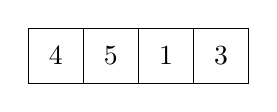
\begin{tikzpicture}[scale=0.7]
\draw (0,0) grid (4,1);

\node at (0.5,0.5) {$4$};
\node at (1.5,0.5) {$5$};
\node at (2.5,0.5) {$1$};
\node at (3.5,0.5) {$3$};
\end{tikzpicture}
\end{center}
suurin pistemäärä on 8.
Aloittajan optimaalinen pelitapa on poistaa ensin luku 3.
Sitten vastustaja poistaa luvun 1 tai 4,
jonka jälkeen aloittaja saa poistettua luvun 5.
Aloittaja saa siis yhteensä $3+5=8$ pistettä.

Poistopelin optimaalisen pelitavan saa selville
dynaamisella ohjelmoinnilla, jossa jokaiselle
taulukon välille lasketaan suurin mahdollinen
aloittajan pistemäärä.
Vastaavalla tavalla voi lähestyä muitakin
pelejä, joissa kerätään pisteitä,
jos tilojen määrä on riittävän pieni.

Huomaa, että ahne strategia, joka poistaa aina
suuremman luvun, ei tuota välttämättä suurinta
pistemäärää. Esimerkiksi yllä olevassa pelissä
ahne strategia tuottaa pistemäärän 7,
vaikka pistemäärä 8 on mahdollinen.

\section{Nim-peli}

Nim-peli on yksinkertainen peli,
joka on tärkeässä asemassa peliteoriassa,
koska monia pelejä voi pelata samalla
strategialla kuin nim-peliä.
Tutustumme aluksi nim-peliin ja yleistämme
strategian sitten muihin peleihin.

\textit{Nim-peli:} Pelissä on $n$ kasaa tikkuja,
joissa kussakin on tietty määrä tikkuja.
Joka vuorolla pelaaja valitsee yhden epätyhjän kasan
ja poistaa siitä minkä tahansa määrän tikkuja.
Pelin voittaa se, joka poistaa viimeisen tikun.

Nim-pelin tila on muotoa $[x_1,x_2,\ldots,x_n]$,
jossa $x_k$ on tikkujen määrä kasassa $k$.
Esimerkiksi $[10,12,5]$ tarkoittaa nim-peliä,
jossa on kolme kasaa ja tikkujen määrät ovat 10, 12 ja 5.
Tila $[0,0,\ldots,0]$ on häviötila,
koska siitä ei voi poistaa mitään tikkua,
ja peli päättyy aina siihen.

\subsection{Analyysi}

Osoittautuu, että nim-pelin tilan luonteen
kertoo xor-summa $x_1 \oplus x_2 \oplus \cdots \oplus x_n$,
missä $\oplus$ tarkoittaa xor-operaatiota.
Jos xor-summa on 0, tila on häviötila,
ja muussa tapauksessa tila on voittotila.
Esimerkiksi tilan $[10,12,5]$ xor-summa on
$10 \oplus 12 \oplus 5 = 3$, joten tila on voittotila.

Mutta miten xor-summa liittyy nim-peliin?
Tämä selviää tutkimalla, miten xor-summa muuttuu,
kun nim-pelin tila muuttuu.

\subsubsection*{Häviötilat}

Pelin päätöstila $[0,0,\ldots,0]$ on häviötila,
ja sen xor-summa on 0, kuten kuuluukin.
Muissa häviötiloissa mikä tahansa siirto johtaa
voittotilaan, koska yksi luvuista $x_k$ muuttuu
ja samalla pelin xor-summa muuttuu
eli siirron jälkeen xor-summasta tulee jokin muu kuin 0.

\subsubsection*{Voittotilat}

Voittotilasta pääsee häviötilaan muuttamalla
jonkin kasan $k$ tikkujen määräksi $x_k \oplus s$,
missä $s$ on pelin xor-summa.
Vaatimuksena on, että $x_k \oplus s < x_k$,
koska kasasta voi vain poistaa tikkuja.
Sopiva kasa $x_k$ on jokin sellainen,
jossa on ykkösbitti samassa kohdassa kuin
$s$:n vasemmanpuoleisin ykkösbitti.

\subsubsection*{Esimerkki}

Tila $[10,12,5]$ on voittotila,
koska sen xor-summa on 3.
Täytyy siis olla olemassa siirto,
jolla tilasta pääsee häviötilaan.
Selvitetään se seuraavaksi.

Pelin xor-summa muodostuu seuraavasti:

\begin{center}
\begin{tabular}{r|r}
10 & \texttt{1010} \\
12 & \texttt{1100} \\
5 & \texttt{0101} \\
\hline
3 & \texttt{0011} \\
\end{tabular}
\end{center}

Tässä tapauksessa
10 tikun kasa on ainoa,
jonka bittiesityksessä on ykkösbitti
samassa kohdassa kuin 
xor-summan vasemmanpuoleisin ykkösbitti:

\begin{center}
\begin{tabular}{r|r}
10 & \texttt{10\textcircled{1}0} \\
12 & \texttt{1100} \\
5 & \texttt{0101} \\
\hline
3 & \texttt{00\textcircled{1}1} \\
\end{tabular}
\end{center}

Kasan uudeksi sisällöksi täytyy saada
$10 \oplus 3 = 9$ tikkua,
mikä onnistuu poistamalla 1 tikku
10 tikun kasasta.
Tämän jälkeen tilanne on:

\begin{center}
\begin{tabular}{r|r}
9 & \texttt{1001} \\
12 & \texttt{1100} \\
5 & \texttt{0101} \\
\hline
0 & \texttt{0000} \\
\end{tabular}
\end{center}

\subsection{Misääripeli}

Misääripelissä nim-pelin tavoite on käänteinen,
eli pelin häviää se, joka poistaa viimeisen tikun.
Osoittautuu, että misääripeliä pystyy pelaamaan lähes samalla
strategialla kuin tavallista nim-peliä.

Ideana on pelata misääripeliä aluksi kuin tavallista
nim-peliä, mutta muuttaa strategiaa pelin
lopussa. Käänne tapahtuu silloin, kun seuraavan
siirron seurauksena kaikissa pelin kasoissa olisi 0 tai 1 tikkua.

Tavallisessa nim-pelissä tulisi nyt tehdä siirto,
jonka jälkeen 1-tikkuisia kasoja on parillinen määrä.
Misääripelissä tulee kuitenkin tehdä siirto,
jonka jälkeen 1-tikkuisia kasoja on pariton määrä.

Tämä strategia toimii, koska käännekohta tulee aina
vastaan jossakin vaiheessa peliä,
ja kyseinen tila on voittotila,
koska siinä on tarkalleen yksi kasa,
jossa on yli 1 tikkua,
joten xor-summa ei ole 0.

\section{Muunnos nimiksi}

Nim-pelin hienoutena on, että mikä tahansa peli,
jossa kaksi pelaajaa tekee siirtoja vuorotellen
ja viimeinen siirto ratkaisee voittajan,
voidaan muuttaa nim-peliksi
ja siinä pystyy käyttämään samaa strategiaa kuin nim-pelissä.
Tämä tulos tunnetaan nimellä Sprague–Grundyn lause.

\subsection{Grundy-luku}

Pelin tilan Grundy-luku on pienin ei-negatiivinen kokonaisluku,
joka ei ole minkään sellaisen tilan Grundy-luku,
johon tilasta pääsee yhdellä siirrolla.
Jos tilasta ei pääse mihinkään tilaan,
sen Grundy-luku on 0.

Grundy-luku vastaa tikkujen määrää nim-kasassa.
Jos Grundy-luku on 0, tilasta pääsee vain tiloihin,
joiden Grundy-luku ei ole 0.
Jos taas Grundy-luku on $x>0$, siitä pääsee tiloihin,
joiden Grundy-luku on $0,1,\ldots,x-1$.

\subsubsection*{Esimerkki}

\textit{Sokkelopeli:} Sokkelossa on pelihahmo,
jota pelaajat siirtävät vuorotellen.
Jokainen sokkelon ruutu on lattiaa tai seinää.
Kullakin siirrolla hahmon tulee liikkua jokin
määrä askeleita vasemmalle tai jokin
määrä askeleita ylöspäin.
Pelin voittaja on se, joka tekee viimeisen siirron.

Esimerkiksi seuraavassa on pelin mahdollinen aloitustilanne,
jossa @ on pelihahmo ja * merkitsee ruutua, johon hahmo voi siirtyä.

\begin{center}
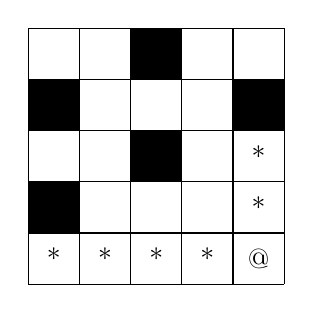
\begin{tikzpicture}[scale=.65]
  \begin{scope}
    \fill [color=black] (0, 1) rectangle (1, 2);
    \fill [color=black] (0, 3) rectangle (1, 4);
    \fill [color=black] (2, 2) rectangle (3, 3);
    \fill [color=black] (2, 4) rectangle (3, 5);
    \fill [color=black] (4, 3) rectangle (5, 4);

    \draw (0, 0) grid (5, 5);
    
    \node at (4.5,0.5) {@};
    \node at (3.5,0.5) {*};
    \node at (2.5,0.5) {*};
    \node at (1.5,0.5) {*};
    \node at (0.5,0.5) {*};
    \node at (4.5,1.5) {*};
    \node at (4.5,2.5) {*};
    
  \end{scope}
\end{tikzpicture}
\end{center}

Sokkelopelin tiloja ovat kaikki sokkelon
lattiaruudut. Äskeisessä esimerkissä
tilojen Grundy-luvut ovat seuraavat:

\begin{center}
\begin{tikzpicture}[scale=.65]
  \begin{scope}
    \fill [color=black] (0, 1) rectangle (1, 2);
    \fill [color=black] (0, 3) rectangle (1, 4);
    \fill [color=black] (2, 2) rectangle (3, 3);
    \fill [color=black] (2, 4) rectangle (3, 5);
    \fill [color=black] (4, 3) rectangle (5, 4);

    \draw (0, 0) grid (5, 5);
    

    \setcounter{row}{5}
    \setrow {0}{1}{}{0}{1}
    \setrow {}{0}{1}{2}{}
    \setrow {0}{2}{}{1}{0}
    \setrow {}{3}{0}{4}{1}
    \setrow {0}{4}{1}{3}{2}
    
  \end{scope}
\end{tikzpicture}
\end{center}

Tämän muunnoksen jälkeen sokkelopelin
tila käyttäytyy
samalla tavalla kuin nim-pelin kasa.
Huomaa, että toisin kuin nim-pelissä,
tilasta saattaa päästä toiseen tilaan,
jonka Grundy-luku on suurempi.
Tällaisen siirron voi kuitenkin
aina peruuttaa niin,
että Grundy-luku palautuu samaksi.

\subsection{Alipelit}

Oletetaan seuraavaksi, että peli muodostuu
alipeleistä ja jokaisella vuorolla
pelaaja valitsee jonkin alipeleistä ja
tekee siirron siinä.
Peli päättyy, kun missään alipelissä ei
pysty tekemään siirtoa.

Nyt pelin tilan Grundy-luku on alipelien
Grundy-lukujen xor-summa.
Peliä pystyy pelaamaan nim-pelin
tapaan selvittämällä kaikkien alipelien Grundy-luvut
ja laskemalla niiden xor-summa.

\subsubsection*{Esimerkki}

Kolmen sokkelon pelissä joka siirrolla pelaaja
valitsee yhden sokkeloista ja siirtää siinä olevaa hahmoa.
Pelin aloitustilanne voi olla seuraavanlainen:

\begin{center}
\begin{tabular}{ccc}
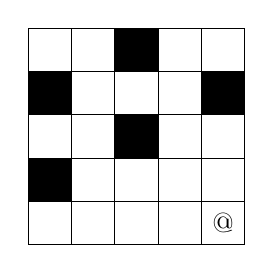
\begin{tikzpicture}[scale=.55]
  \begin{scope}
    \fill [color=black] (0, 1) rectangle (1, 2);
    \fill [color=black] (0, 3) rectangle (1, 4);
    \fill [color=black] (2, 2) rectangle (3, 3);
    \fill [color=black] (2, 4) rectangle (3, 5);
    \fill [color=black] (4, 3) rectangle (5, 4);

    \draw (0, 0) grid (5, 5);

    \node at (4.5,0.5) {@};

    \end{scope}
\end{tikzpicture}
&
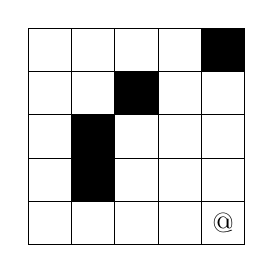
\begin{tikzpicture}[scale=.55]
  \begin{scope}
    \fill [color=black] (1, 1) rectangle (2, 3);
    \fill [color=black] (2, 3) rectangle (3, 4);
    \fill [color=black] (4, 4) rectangle (5, 5);

    \draw (0, 0) grid (5, 5);
    
    \node at (4.5,0.5) {@};

  \end{scope}
\end{tikzpicture}
&
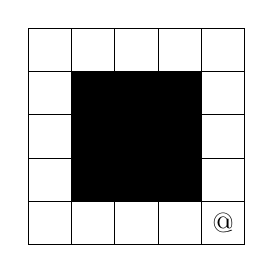
\begin{tikzpicture}[scale=.55]
  \begin{scope}
    \fill [color=black] (1, 1) rectangle (4, 4);

    \draw (0, 0) grid (5, 5);
    
    \node at (4.5,0.5) {@};
  \end{scope}
\end{tikzpicture}
\end{tabular}
\end{center}

Sokkeloiden ruutujen Grundy-luvut ovat:

\begin{center}
\begin{tabular}{ccc}
\begin{tikzpicture}[scale=.55]
  \begin{scope}
    \fill [color=black] (0, 1) rectangle (1, 2);
    \fill [color=black] (0, 3) rectangle (1, 4);
    \fill [color=black] (2, 2) rectangle (3, 3);
    \fill [color=black] (2, 4) rectangle (3, 5);
    \fill [color=black] (4, 3) rectangle (5, 4);

    \draw (0, 0) grid (5, 5);

    \setcounter{row}{5}
    \setrow {0}{1}{}{0}{1}
    \setrow {}{0}{1}{2}{}
    \setrow {0}{2}{}{1}{0}
    \setrow {}{3}{0}{4}{1}
    \setrow {0}{4}{1}{3}{2}

    \end{scope}
\end{tikzpicture}
&
\begin{tikzpicture}[scale=.55]
  \begin{scope}
    \fill [color=black] (1, 1) rectangle (2, 3);
    \fill [color=black] (2, 3) rectangle (3, 4);
    \fill [color=black] (4, 4) rectangle (5, 5);

    \draw (0, 0) grid (5, 5);

    \setcounter{row}{5}
    \setrow {0}{1}{2}{3}{}
    \setrow {1}{0}{}{0}{1}
    \setrow {2}{}{0}{1}{2}
    \setrow {3}{}{1}{2}{0}
    \setrow {4}{0}{2}{5}{3}    
    
  \end{scope}
\end{tikzpicture}
&
\begin{tikzpicture}[scale=.55]
  \begin{scope}
    \fill [color=black] (1, 1) rectangle (4, 4);

    \draw (0, 0) grid (5, 5);

    \setcounter{row}{5}
    \setrow {0}{1}{2}{3}{4}
    \setrow {1}{}{}{}{0}
    \setrow {2}{}{}{}{1}
    \setrow {3}{}{}{}{2}
    \setrow {4}{0}{1}{2}{3}    
    
  \end{scope}
\end{tikzpicture}
\end{tabular}
\end{center}

Aloitustilanteessa Grundy-lukujen xor-summa on
$2 \oplus 3 \oplus 3 = 2$, joten
aloittaja pystyy voittamaan pelin.
Sopiva aloitussiirto on liikkua vasemmassa sokkelossa
2 askelta ylöspäin, jolloin xor-summaksi
tulee $0 \oplus 3 \oplus 3 = 0$.

\subsection{Jakautuminen}

Joskus pelissä on joukko alipelejä,
joista jokainen voi jakautua uusiksi alipeleiksi.
Kuten ennenkin, jokainen alipeli vastaa
nim-pelin kasaa ja alipelien joukon Grundy-luku
saadaan laskemalla xor-summa alipelien Grundy-luvuista.

Alipelin Grundy-luku selviää käymällä
läpi kaikki tavat, miten alipeli voi jakautua.
Jokainen jakotapa luo alipelien joukon,
jonka Grundy-luvun saa laskettua xor-summalla.
Alipelin Grundy-luku on pienin luku,
joka ei ole mikään näistä xor-summista.
Sama jatkuu rekursiivisesti pienempiin alipeleihin.

\subsubsection*{Esimerkki}

Tarkastellaan lopuksi seuraavaa peliä:

\textit{Bittipeli:} Annettuna on joukko
bittijonoja. Joka vuorolla pelaaja valitsee
jonkin bittijonon ja jakaa sen kahteen
osaan niin, että kumpaankin osaan
jää sekä bitti 0 että bitti 1.
Pelin voittaja on se, joka tekee viimeisen siirron.

Esimerkiksi pelissä $\{1101001\}$
on kolme mahdollista siirtoa, jotka tuottavat
alipelit $\{110,1001\}$, $\{1101,001\}$ ja $\{11010,01\}$.
Pelin Grundy-luku on pienin kokonaisluku,
joka ei ole minkään alipelin Grundy-luku.

Alipelin $\{110,1001\}$ Grundy-luku on
alipelien $\{110\}$ ja $\{1001\}$ Grundy-lukujen
xor-summa. Alipelin $\{110\}$ Grundy-luku on 0,
koska mitään siirtoa ei voi tehdä.
Alipelin $\{1001\}$ Grundy-luku on 1,
koska ainoa siirto luo alipelin $\{10,01\}$,
jonka Grundy-luku on 0.
Niinpä alipelin $\{110,1001\}$ Grundy-luku on $0 \oplus 1 = 1$.

Vastaavasti saadaan, että
alipelien $\{1101,001\}$ ja $\{11010,01\}$
Grundy-luvut ovat 0 ja 1.
Pelin $\{1101001\}$ Grundy-luku on siis 2,
koska siinä on kolme mahdollista siirtoa,
jotka tuottavat alipelit, joiden Grundy-luvut
ovat 1, 0 ja 1.

Tässä tapauksessa aloittaja voittaa
jakamalla bittijonon $\{1101,001\}$. Tämän jälkeen vastustaja
ei voi tehdä mitään siirtoa ja peli on päättynyt.

%\endinput

